\documentclass{beamer}

\usecolortheme[light]{solarized}

\beamertemplatenavigationsymbolsempty
\usepackage[utf8]{inputenc}

\usepackage{hyperref}
\usepackage{minted}
\usepackage{booktabs}
\usepackage{standalone}

\usepackage{graphicx}
\usepackage{tikz}
\usetikzlibrary{arrows}
\usetikzlibrary{decorations.markings}
\usetikzlibrary{calc, patterns}
\usetikzlibrary{shapes,snakes}

\begin{document}

    \begin{frame}
        \begin{center}
            \Huge

            Maths saves lives 

            \Large
            Operational research for healthcare

            \vspace{1cm}

            School of Mathematics

            \normalsize
            Vince Knight
        \end{center}
    \end{frame}

    \begin{frame}[fragile]
        \frametitle{Data}
        \begin{center}
            \begin{tabular}{llrr}
                \toprule
                & Sex & Height & Weight \\
                \midrule
                0 & M & 187.306088 & 72.233276 \\
                1 & M & 170.595112 & 92.195728 \\
                2 & F & 157.637346 & 64.835601 \\
                3 & M & 162.010640 & 130.462244 \\
                4 & F & 154.017198 & 81.568846 \\
                $\vdots$ & $\vdots$ & $\vdots$ & $\vdots$ \\
                \bottomrule
            \end{tabular}
            \vspace{1cm}
            \pause
            \small{
                \begin{minted}{python}
      >>> import scipy.stats

      >>> ttest = scipy.stats.ttest_ind(
      ...    df[df['Sex']=='M']['Height'],
      ...    df[df['Sex']=='F']['Height'])
      >>> ttest.pvalue
      0.070033630470421021
                \end{minted}
            }
        \end{center}
\end{frame}

    \begin{frame}
        \begin{center}
            \Huge
            Examples

			\normalsize
			(Geraint Palmer)
        \end{center}
    \end{frame}

\frame{
  \frametitle{Optimisation}
  \begin{center}
		\begin{tabular}{lcccccccccc}
			\toprule
		Shift & 9 & 10 & 11 & 12 & 13 & 14 & 15 & 16 & 17 & 18\\
			\midrule
		Nurses & 7 & 8 & 9 & 9 & 7 & 5 & 4 & 8 & 4 & 3\\
			\bottomrule
		\end{tabular}

      \vspace{10mm}
      \includestandalone[width=0.4\textwidth]{./img/fulltime}
      \hspace{10mm}
      \includestandalone[width=0.4\textwidth]{./img/parttime}
  \end{center}
}

\frame{
  \frametitle{Graph Theory}
  \begin{center}
    \includestandalone[width=0.9\textwidth]{./img/rhondda_gt}
  \end{center}
}

\frame{
  \begin{center}
      \includestandalone[width=0.85\textwidth]{./img/rhondda_graph}
  \end{center}
}

    \begin{frame}
		\frametitle{Queueing Theory}
        \begin{center}
            
\begin{tikzpicture}

                \node (I1) at (0, 0) [draw, circle, fill=blue!50] {};
                \node (I2) at ($(I1) + (0.5, 0)$) [draw, circle, fill=blue!50] {};
                \node (I3) at ($(I2) + (0.5, 0)$) [draw, circle, fill=blue!50] {};
                \node (I4) at ($(I3) + (0.5, 0)$) [draw, circle, fill=blue!50] {};

                \draw ($(I1) + (-1.25, 0)$) -- ($(I1) + (-.25, 0)$) [->, thick] ;
                \node at ($(I1) + (-1.25, 0)$) [left] {every time unit};

                \draw [thick] ($(I4) + (0.5, 0.25)$) --
                              ($(I4) + (0.5, -0.25)$) --
                              ($(I4) + (1.5, -0.25)$) --
                              ($(I4) + (1.5, 0.25)$);

                \node (I5) at ($(I4) + (1, 0)$) [draw, circle, fill=red!50] {};

                \draw ($(I5) + (.5, 0)$) -- ($(I5) + (1.5, 0)$) [->, thick];
                \node at ($(I5) + (1.5, 0)$) [right] {every time unit};


            \end{tikzpicture}
        \end{center}
    \end{frame}

\begin{frame}
    \begin{center}
        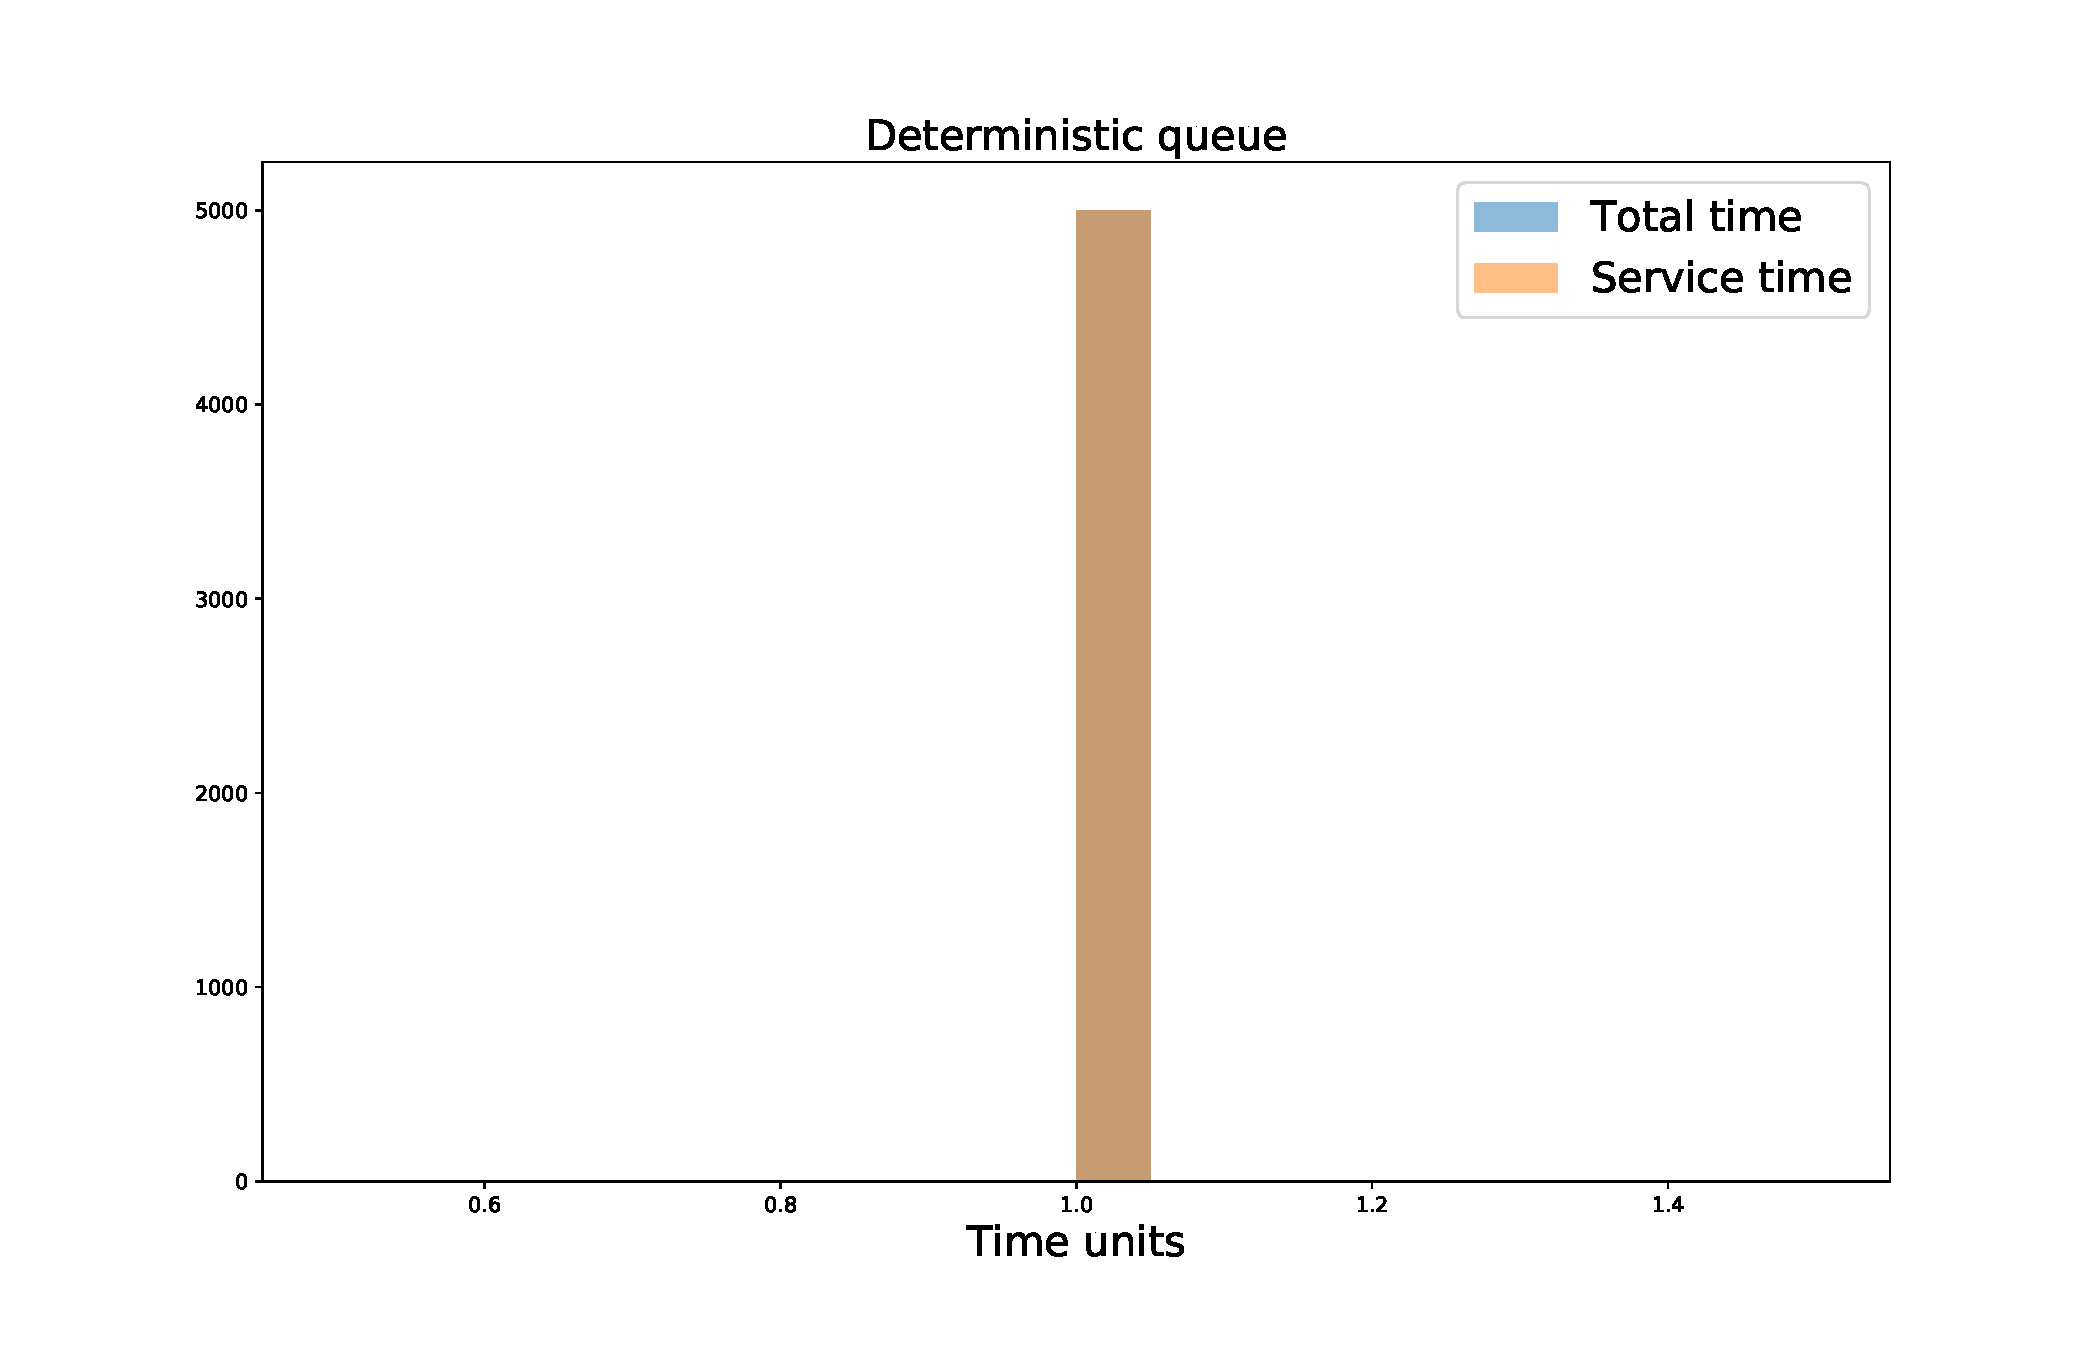
\includegraphics[width=\textwidth]{./img/deterministic_queue.pdf}
    \end{center}
\end{frame}

\begin{frame}
    \begin{center}
        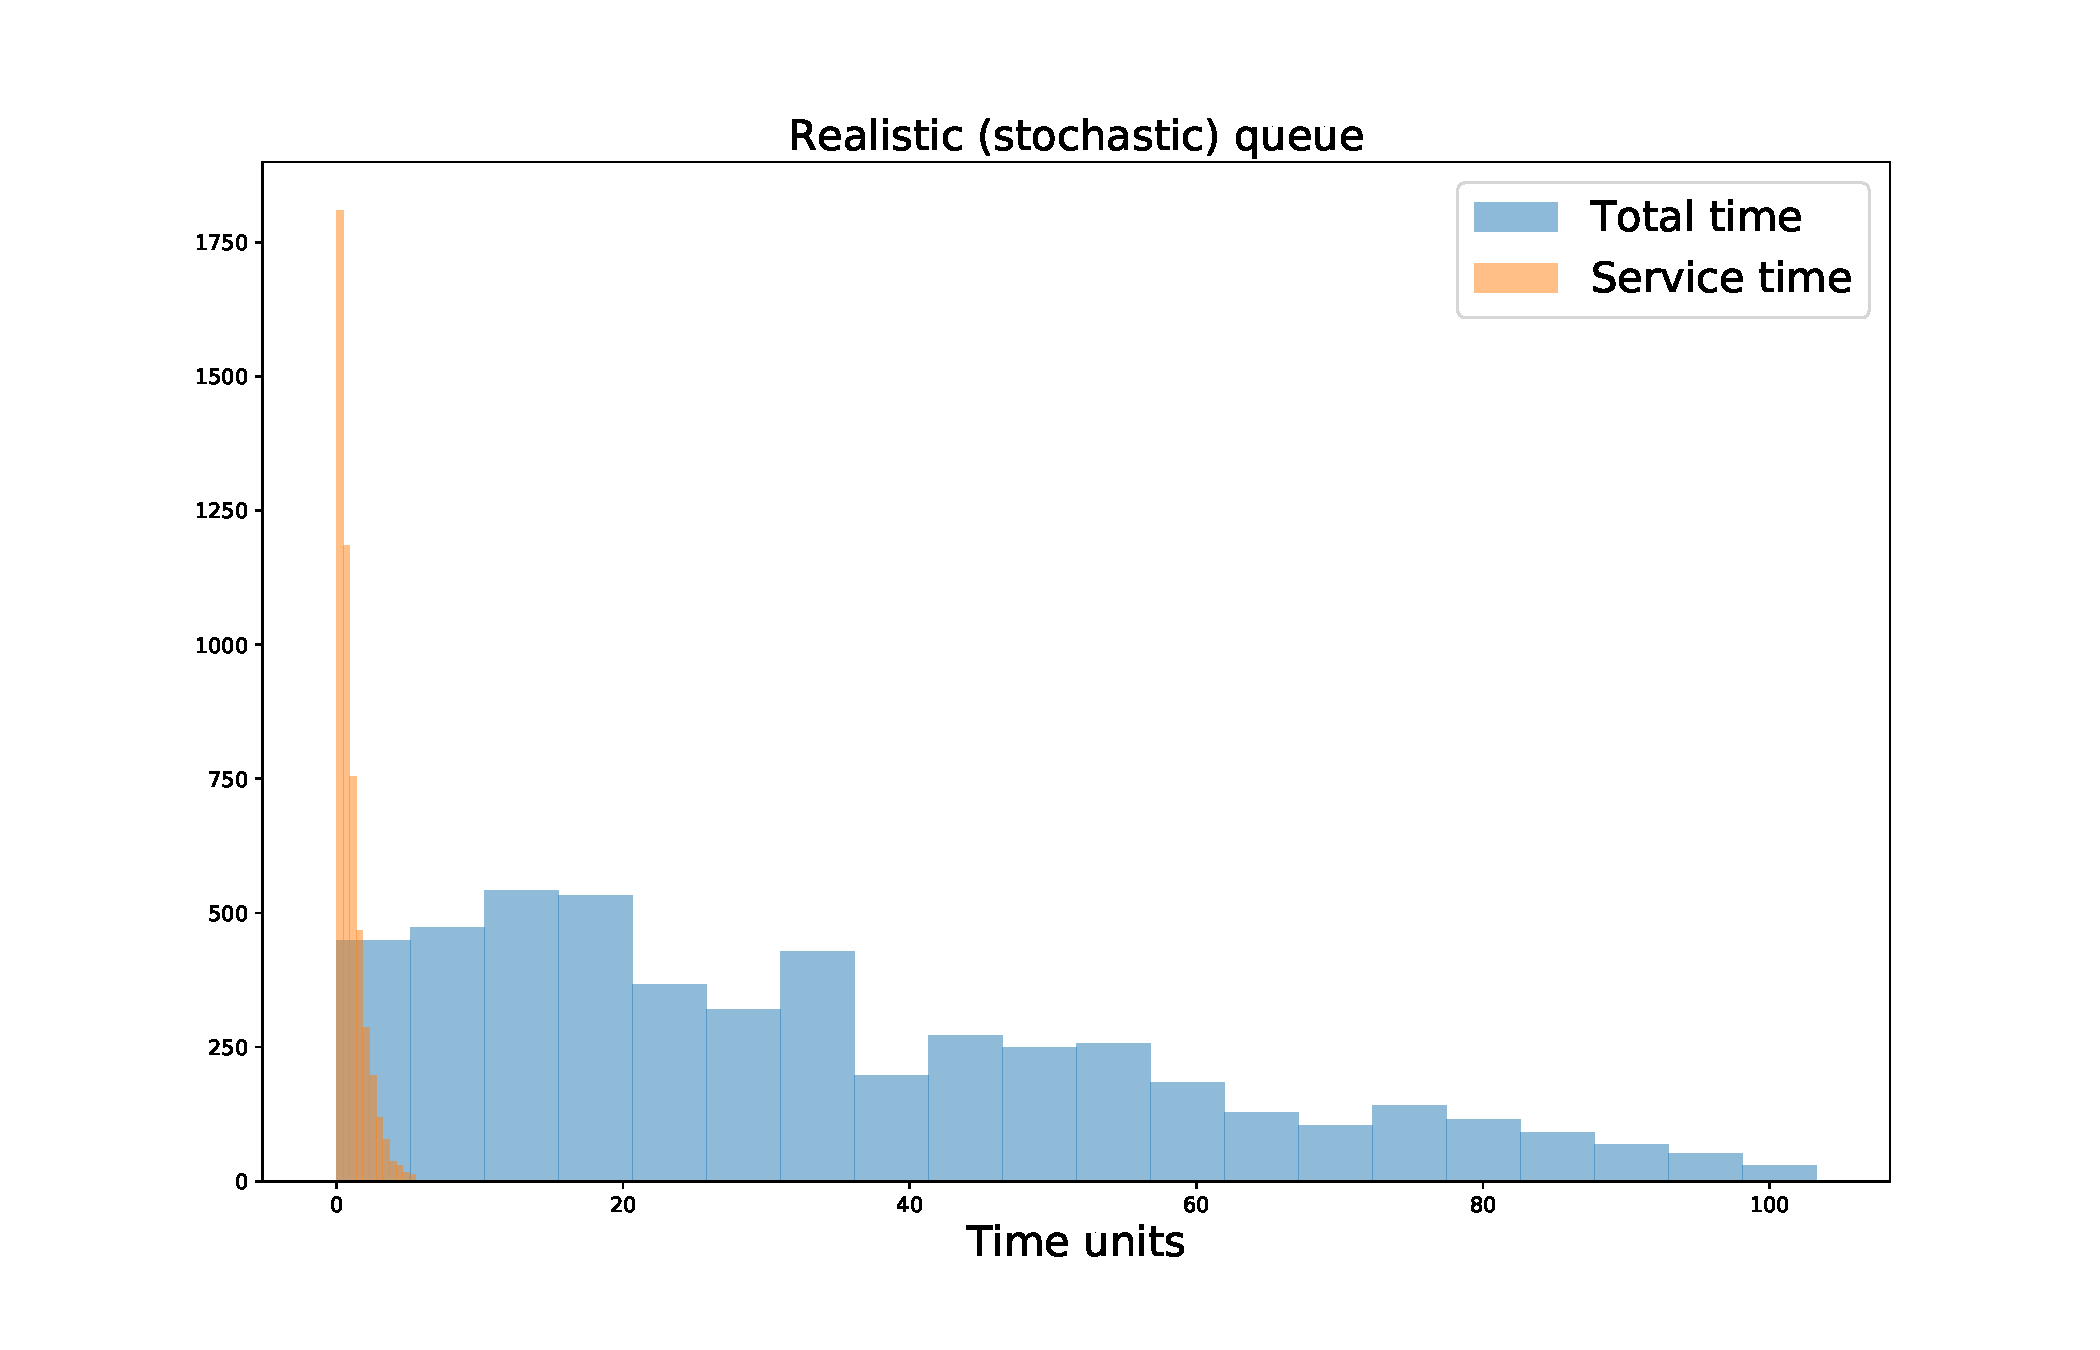
\includegraphics[width=\textwidth]{./img/stochastic_queue.pdf}
    \end{center}
\end{frame}

\frame{
  \frametitle{Dynamical Systems}
  \begin{center}
    \includestandalone[width=\textwidth]{./img/sir}
  \end{center}
}


\begin{frame}
	\begin{center}
	  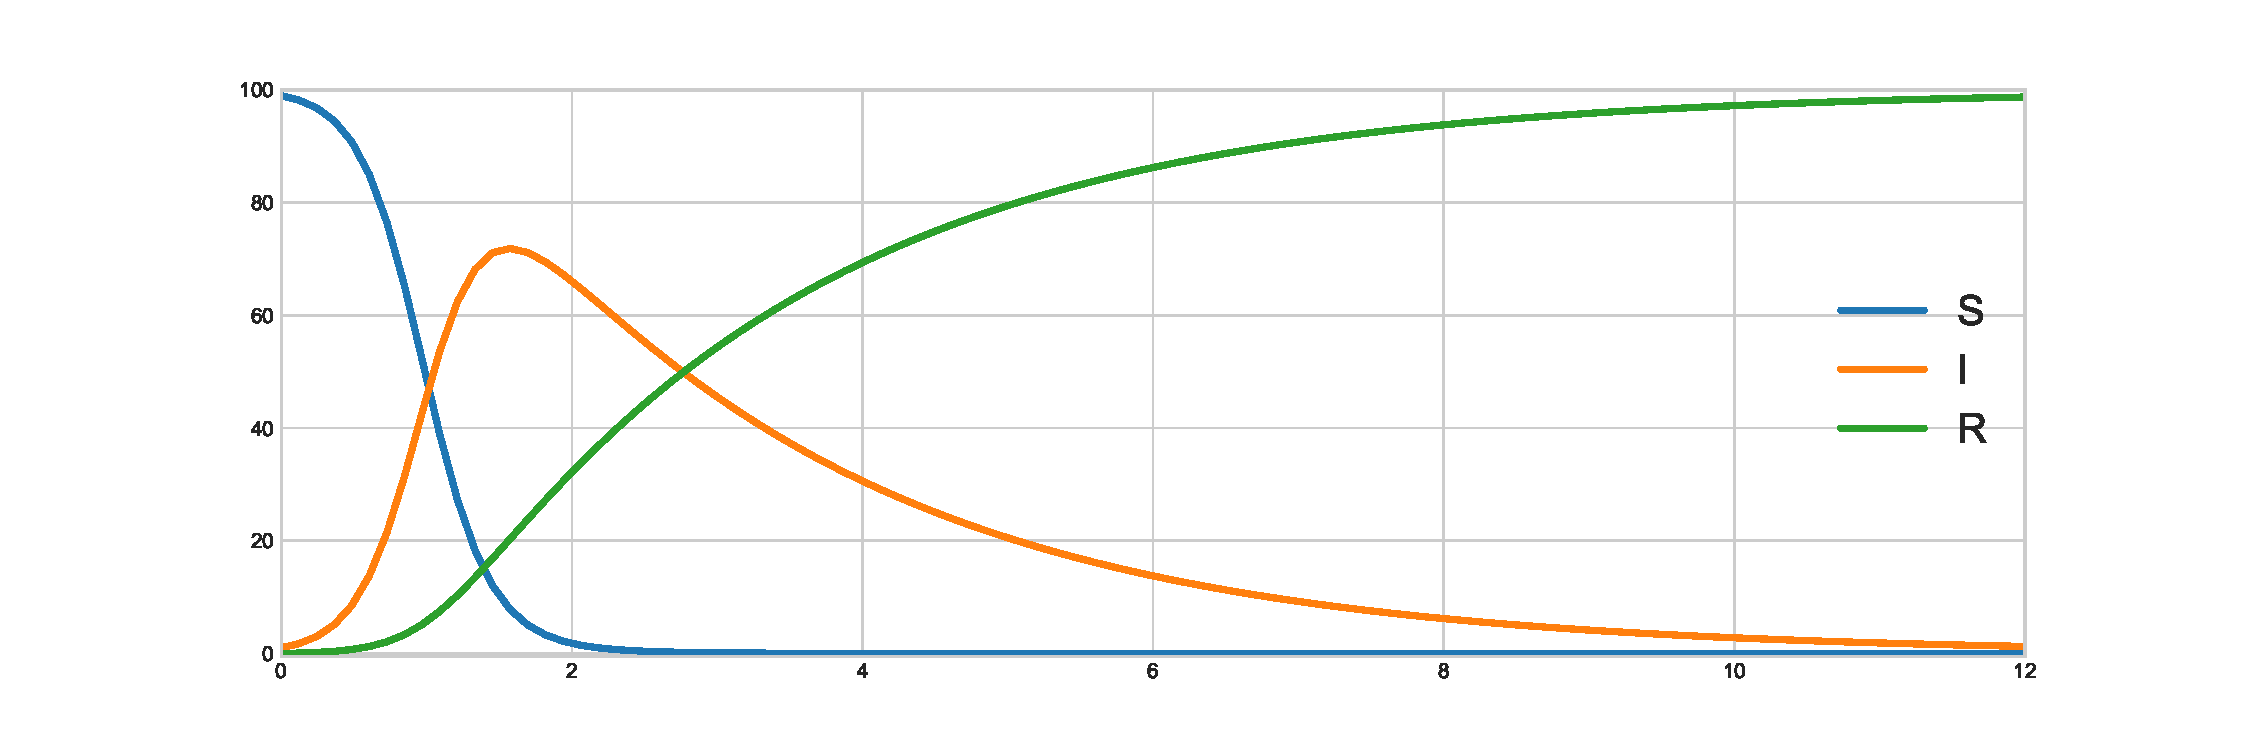
\includegraphics[width=0.9\textwidth]{./img/SIR.pdf}
	\end{center}
\end{frame}

\frame{
  \frametitle{Game Theory}
  \includestandalone[width=\textwidth]{./img/hospitals}
}

    \begin{frame}
        \begin{center}
            \Huge
            Partnerships
        \end{center}
    \end{frame}

	\begin{frame}
		\begin{center}
			\Huge
			Welsh Ambulance Service Trust
		\end{center}
	\end{frame}

\begin{frame}
\begin{center}
	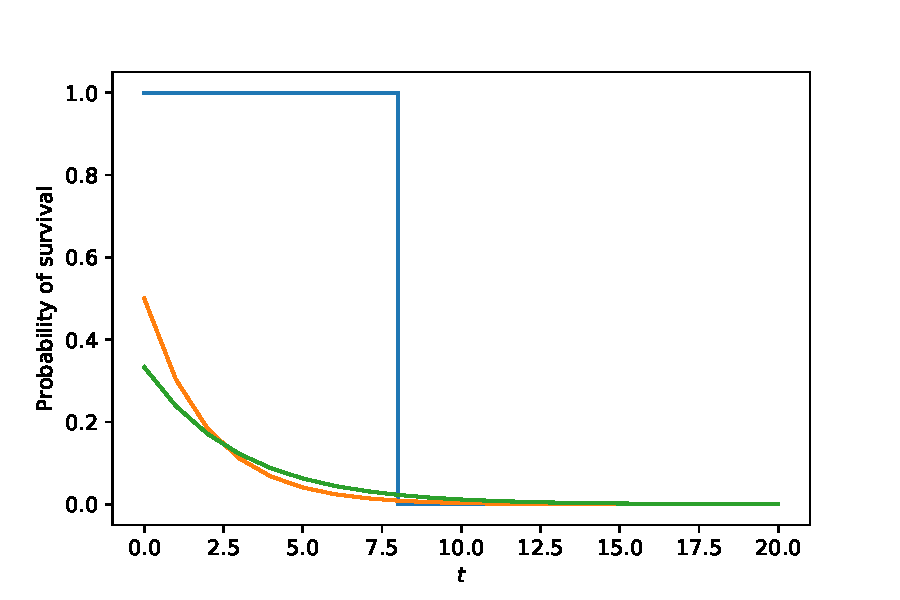
\includegraphics[width=.8\textwidth]{./img/survival_plot.pdf}
\end{center}

\textit{Ambulance allocation for maximal survival with heterogeneous outcome measures}
V.A. Knight, P.R. Harper, L. Smith (2012) \textbf{Omega}
\end{frame}


	\begin{frame}
		\begin{center}
			\Huge
			University Hospital of Wales (UHW)
		\end{center}
	\end{frame}

\begin{frame}

\begin{center}
	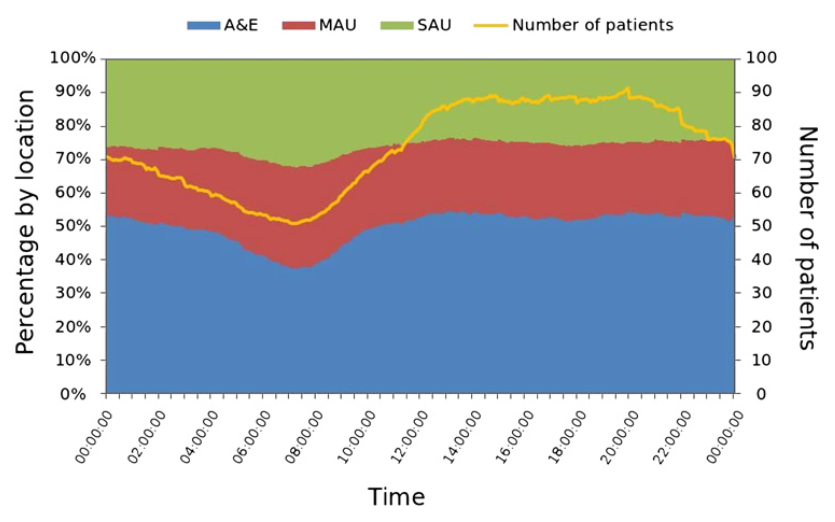
\includegraphics[width=.8\textwidth]{./img/eu_work.png}
\end{center}

\textit{How efficient can an emergency unit be? A perfect world model.}
Kesh Baboolal, Jeff D Griffiths, Vincent A Knight, Andrew V Nelson, Cheryl Voake, Janet E Williams (2012) \textbf{EMJ}
\end{frame}

	\begin{frame}
		\begin{center}
			\Huge
			Aneurin Bevan University Health Board
		\end{center}
	\end{frame}

	\begin{frame}
\begin{center}
	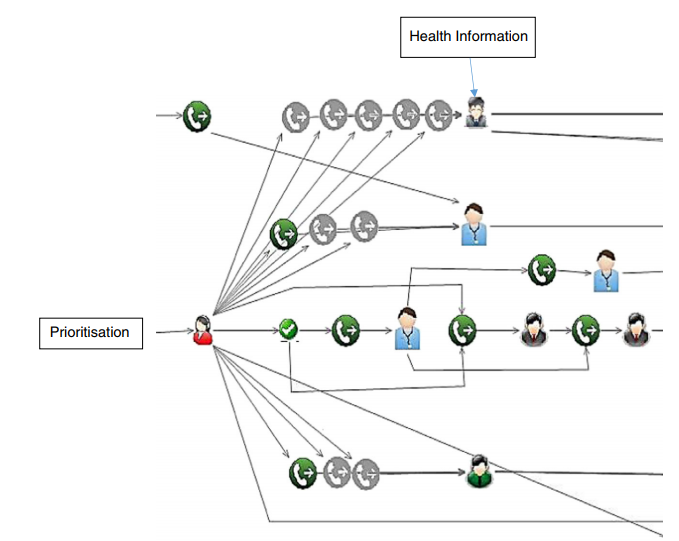
\includegraphics[width=.7\textwidth]{./img/111_work.png}
\end{center}

\textit{Modelling for the proposed roll-out of the ‘111’ service in Wales:
a case study} Mark Tuson,  Tracey England, Doris Behrens, Richard Bowen,
Dorothy Edwards, John Frankish, Jude Kay (2016) \textbf{Health Care Management Science}
	\end{frame}

	\begin{frame}
		\begin{center}
			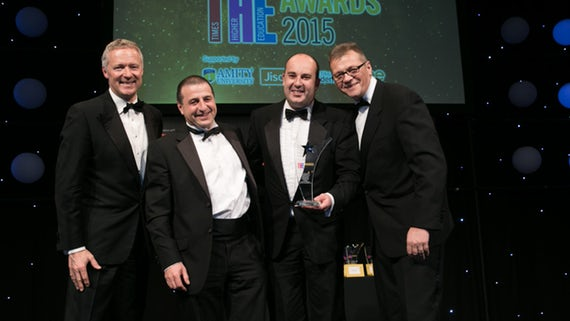
\includegraphics[width=.8\textwidth]{./img/the-awards.jpg}
		\end{center}
	\end{frame}

	\begin{frame}
		\begin{center}
			\Huge
			M.Sc.
		\end{center}
	\end{frame}

    \begin{frame}
        \Large
        \begin{itemize}
            \item \texttt{knightva@cardiff.ac.uk}
            \item \texttt{harper@cardiff.ac.uk}
            \item \texttt{emeryjl4@cardiff.ac.uk}
        \end{itemize}
    \end{frame}

\end{document}
